\documentclass[11pt]{article}
\usepackage[paperwidth=30cm,paperheight=30cm,margin=5mm]{geometry}
\usepackage[T1]{fontenc}
\usepackage{tikz}
\usetikzlibrary{arrows.meta,positioning,fit,backgrounds,calc,shapes.geometric}
\pagestyle{empty}
\tikzset{
  box/.style={draw, rounded corners=2pt, align=center, font=\small, minimum height=9mm, inner sep=4pt, fill=white},
  data/.style={box, fill=blue!8},
  model/.style={box, fill=orange!12},
  outp/.style={box, fill=green!10},
  frozen/.style={box, dashed, font=\small\itshape},
  arr/.style={-{Latex[length=2mm]}, semithick},
  lbl/.style={font=\scriptsize, align=center},
  group/.style={draw, rounded corners=4pt, dashed, gray, inner sep=6pt},
  glbl/.style={font=\scriptsize\itshape, gray, anchor=south west, inner sep=1pt}}
\begin{document}

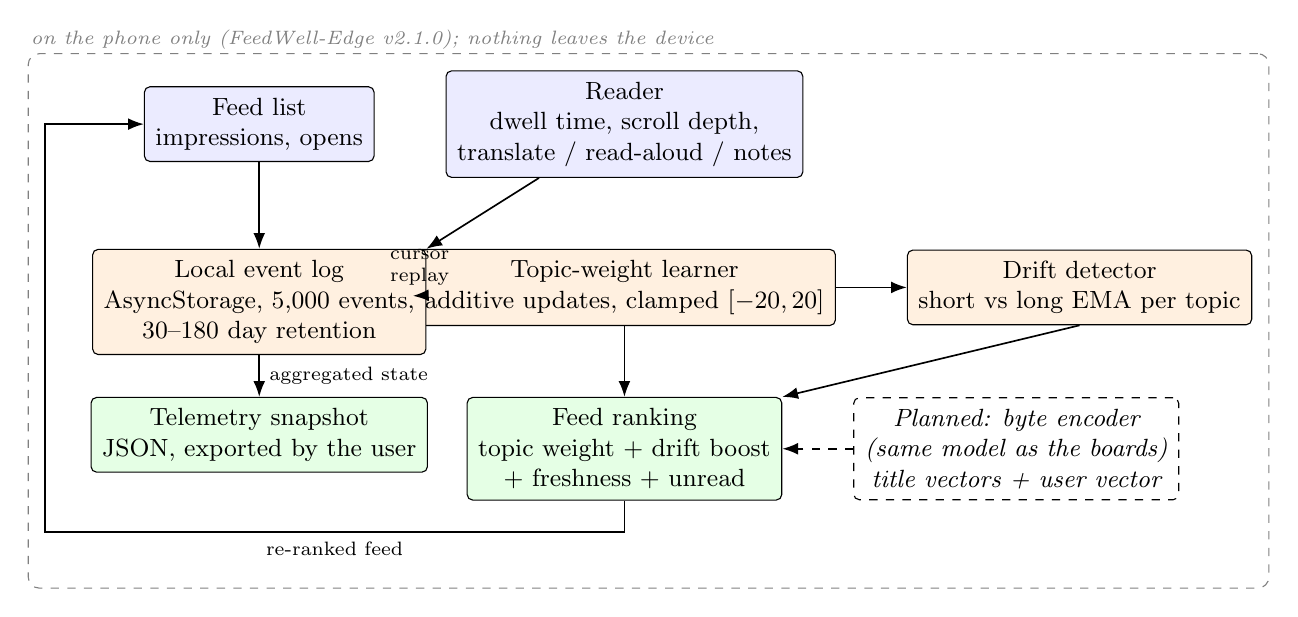
\begin{tikzpicture}[node distance=7mm and 9mm]
  \node[data] (feed) {Feed list\\impressions, opens};
  \node[data, right=of feed] (reader) {Reader\\dwell time, scroll depth,\\translate / read-aloud / notes};
  \node[model, below=9mm of reader] (learn) {Topic-weight learner\\additive updates, clamped $[-20, 20]$};
  \node[model, anchor=north] (log) at (feed.south |- learn.north) {Local event log\\AsyncStorage, 5,000 events,\\30--180 day retention};
  \node[model, right=of learn] (drift) {Drift detector\\short vs long EMA per topic};
  \node[outp, below=9mm of learn] (rank) {Feed ranking\\topic weight + drift boost\\+ freshness + unread};
  \node[outp, anchor=north] (export) at (log.south |- rank.north) {Telemetry snapshot\\JSON, exported by the user};
  \node[frozen, right=of rank] (future) {Planned: byte encoder\\(same model as the boards)\\title vectors + user vector};
  \draw[arr] (feed) -- (log);
  \draw[arr] (reader) -- (log.north east);
  \draw[arr] (log) -- node[lbl, above] {cursor\\replay} (learn);
  \draw[arr] (learn) -- (drift);
  \draw[arr] (learn) -- (rank);
  \draw[arr] (drift.south) -- (rank.north east);
  \draw[arr] (log) -- node[lbl, right] {aggregated state} (export);
  \draw[arr, dashed] (future) -- (rank);
  \coordinate (lm) at ([xshift=-6mm]log.west);
  \coordinate (fb1) at ([yshift=-4mm]rank.south);
  \coordinate (fb2) at (lm |- fb1);
  \coordinate (fb3) at (lm |- feed.west);
  \coordinate (fb4) at ([yshift=-5mm]fb2);
  \draw[arr] (rank.south) -- (fb1) -- node[lbl, below] {re-ranked feed} (fb2) -- (fb3) -- (feed.west);
  \begin{scope}[on background layer]
    \node[group, fit=(feed)(reader)(log)(learn)(drift)(rank)(export)(future)(fb2)(fb4), label={[glbl]north west:on the phone only (FeedWell-Edge v2.1.0); nothing leaves the device}] {};
  \end{scope}
\end{tikzpicture}
\end{document}
